\documentclass[12pt,a4paper]{article}
\usepackage{graphicx}

\usepackage[utf8]{inputenc}
\usepackage[english, spanish]{babel}

\usepackage{wrapfig}
\usepackage{amsmath}
\usepackage{mathtools}
\usepackage{amsfonts}
\usepackage{amssymb}
\usepackage{graphicx}
\usepackage{url}

\usepackage[font=small,format=plain,labelfont=bf,up,textfont=it,up]{caption}
\usepackage{diagbox}
\providecommand{\abs}[1]{\lvert#1\rvert}
\newcommand{\grad}{^{\circ}}


\usepackage[makeroom]{cancel}
\usepackage{enumitem}
\usepackage{float}	
\usepackage{setspace}



\usepackage{subfigure}


\usepackage[export]{adjustbox}

\usepackage{booktabs}
\usepackage{bigstrut}
\usepackage{multirow}
\usepackage{array}
\usepackage{tabularx}
\usepackage{lipsum}  
\usepackage{sectsty}
\usepackage{titlesec}
\usepackage{verbatim}
\usepackage{natbib}



\usepackage{lscape}
\usepackage{tabu}

\usepackage{array}
\newcolumntype{P}[1]{>{\centering\arraybackslash}p{#1}}

\usepackage{xcolor}
\definecolor{dark}{rgb}{0.10,0.2,0.3}
\definecolor{seablue}{rgb}{0.10,0.2,0.45}
\definecolor{light}{rgb}{1.7,1.5,0.6}
\definecolor{purpure}{rgb}{0.5,0.15,0.3}
\definecolor{bluegreen}{rgb}{0.2,0.65,0.65}
\definecolor{bluegreen2}{rgb}{0.2,0.45,0.45}
\definecolor{vcromo}{rgb}{0.0,0.18,0.39}
\usepackage{hyperref}
\hypersetup{colorlinks,%
citecolor=dark,%
filecolor=dark,%
linkcolor=bluegreen,%
urlcolor=purpure}


 
\usepackage[left=3cm,right=3cm,top=2.5cm,bottom=2.5cm]{geometry}

% \titleformat{\section}
%  {\normalfont\sffamily\bfseries\Large\color{vcromo}}
%   {\thesection}{1em}
%   {\sectionrule{25pt}{0.8pt}{-12pt}{0.8pt}}
  
\titleformat{\section}[frame]
{\normalfont\sffamily\bfseries\Large\color{vcromo}}{\filcenter\small
\ FASE \thesection \ }
{10pt}{\LARGE\bfseries\filcenter}

  
\titleformat{\subsection}
  {\normalfont\itshape\large\bfseries\color{dark}}
  {\thesubsection}{1em}{}

% \captionsetup[table]{name=Tabla}

\setcounter{secnumdepth}{5}
\setcounter{tocdepth}{5}

\providecommand{\abs}[1]{\lvert#1\rvert}
\providecommand{\norm}[1]{\lVert#1\rVert}


\begin{document}
%------Portada--------------%
	\begin{titlepage}
	\centering
    {
\includegraphics[width=0.3\textwidth]{fotos/Logo_azul.png}\par}
	\vspace{1cm}
	{\bfseries\LARGE Universidad Politécnica de Madrid \par}
	\vspace{1cm}
	{\scshape\Large Escuela Técnica Superior de Ingenieros Industriales \par}
	\vspace{2.5cm}
	{\scshape\Huge Programación de Sistemas \par}
	\vspace{0.5cm}
	{\scshape\large Departamento de Electrónica y Automática \par}
	\vspace{2cm}
    {\itshape\LARGE Práctica 1: Diseño de un experimento \par}
    \vspace{0.5cm}
    {\upshape\large Implementación y comparación de un generador dinámico de laberintos en C++ mediante un algoritmo \textit{recursivo} e \textit{iterativo}}
	\vfill
	{\large{Celia \textsc{Ramos Ramírez} (18295)\par}}
	\vspace{0.1cm}
    {\large{Gonzalo \textsc{Quirós Torres} (17353)\par}}
	\vspace{0.1cm}
	{\large{Josep María \textsc{Barberá Civera} (17048)\par}}
	\vfill
	{\Large{ $3\grad$ \textsc{GITI}}\par}
	\vfill
	{\Large \today \par}
	\end{titlepage}
	
%-----Página en blaco------%
% \newpage
% \begin{center}
% \textit{\{Esta página se ha dejado intencionadamente en blanco\}}
% \end{center}
% \thispagestyle{empty} %	
% \newpage

\section*{Resumen}
El objetivo del presente trabajo es elaborar y comparar dos algoritmos, uno iterativo y uno recursivo, que realicen una misma acción. Posteriormente se valorará el desempeño de cada uno por separado y se hará una comparación. 

Para que la comparación se haga homogéneamente se ha puesto especial cuidado en que los dos algoritmos, tanto el recursivo como el iterativo, sigan procesos análogos. Para lograrlo el esquema funcional de los algoritmos es prácticamente el mismo, los pasos que sigue el proceso son idénticos salvo por las diferencias inherentes a la naturaleza de los algoritmos y el número de llamadas a ficheros externos desde cada fichero es igual en ambos casos. 

La elaboración de los dos algoritmos no ha sido simultánea: en primer lugar, se elaboró el algoritmo recursivo pues la naturaleza del problema era abordable de forma directa desde la perspectiva de la recursividad. Después se elaboró el algoritmo iterativo, que planteó gran número de dificultades que poco a poco lograron ser salvadas. En último término se adecuó el algoritmo iterativo para que su estructura y forma coincidiera lo más exactamente con el algoritmo recursivo
%------Índice--------------%
{
 \hypersetup{linkcolor=black}%Fijaros que estoy cambiando el color solo localmente...es genial para mantener los liks pero que no sea muy cargante el color para el índice de contenidos!!!
 
 \tableofcontents
}

\pagenumbering{Roman}
\clearpage

%Si quieres que aparezca en el indice de contenidos pero sin numeración, poner lo siguiente simpre después de algún apartado
%\phantomsection
%\addcontentsline{toc}{subsection}{Manolo el del bombo}


\section*{Introducción}
\pagenumbering{arabic}
Los algoritmos recursivos son una potente herramienta para la algoritmia en la programación. En esta memoria se pretende comparar un algoritmo recursivo con otro iterativo. Dicha comparación se realiza mediante el diseño de un experimento el cual pone en evidencia las ventajas y problemáticas que presenta la programación recursiva frente a la iterativa.

La memoria se estructura en cuatro partes que corresponden a las fases seguidas en el experimento.
La primera fase es la de \textit{Ideación}. Es la parte más importante, pues ella condiciona todas las fases posteriores. En ella se plantean las ideas propuestas y se discute la que finalmente ha sido elegida. Además, incluye la implementación sucesiva de los dos algoritmos mediante programación en C++.
La segunda fase en la de \textit{Experimentación}. Es aquí donde se exponen y discuten los criterios de comparación utilizados y cómo se han implementado dichas métricas en el código. Por otro lado, se explica la metodología empleada para las pruebas o toma de mediadas.
La tercera fase es la de \textit{Análisis}. Esta parte resulta de vital importancia y es en ella en la que se pone de manifiesto de forma gráfica los resultado obtenidos en las fases precedentes. Para la realización del análisis heurístico, se ha procedido con ayuda de la herramienta \textsc{RStudio}, a un análisis gráfico.
En la cuarta y última fase de \textit{Conclusiones} se recapitula y enuncian los hechos más relevantes del experimento realizado.

\section{Ideación}
\subsection{Primeras propuestas}

Inicialmente, se pensó en realizar un experimento con esencia matemática, esto es, abordar la resolución de integrales sencillas mediante sumas de Riemann. La inteción era ir variando las particiones del dominio de integración mientras se comparaba el desempeño de los dos algoritmos. Aunque parecía un experimento adecuado, planteaba también varias problemáticas: 

\begin{itemize}
	\item Las funciones han de ser predeterminadas por el programador, perdiendo así la interacción con el usuario.
	\item De lo anterior se desprende que la cantidad de funciones que se pueden muestrear es limitada, lo que puede generar un sesgo, pues las funciones elegidas pueden favorecer el desempeño de un algoritmo frente al otro. 
	\item Otra forma de abordar el problema sería mediante aproximaciones polinómicas a las integrales. Esto supone que las problemáticas anteriores siguen estando presentes, pero, además, las fórmulas de aproximación polinómica son sencillas (hasta cierto grado) y por ende los tiempos de ejecución no serían suficientemente largos para que la comparación resultare significativa. 
\end{itemize}

Como segunda posibilidad se valoró la implementación de \textit{juegos de estrategia} como el tres en raya, cuatro en raya, etc. Pero se dedujo que en un tablero acotado como en el tres en raya las iteraciones iban a ser siempre las mismas y al mismo tiempo no tenía sentido diseñar un tablero más grande pues el problema se iba a concentrar en un espacio reducido.

Finalmente se encontró otros algoritmos que diseñaban laberintos a partir de una malla rellena por carácteres. De entre los distintos métodos que abordaban el problema, se eligió aquel que consistía en visitar una por una las casillas, comprobando si eran válidas e ir abriéndose camino hasta rellenar toda la malla con pasillos. Esta metodología es conocida como \textit{recursive backtracker}\cite{wiki}. El cual es una versión aleatoriazada del algoritmo \textit{depht first-first search}. En la siguiente ilustración (ver \textsc{Fig.}~\ref{back_tracker}) puede verse un ejemplo del algoritmo implementado.

\begin{figure}[H]
	\centering
	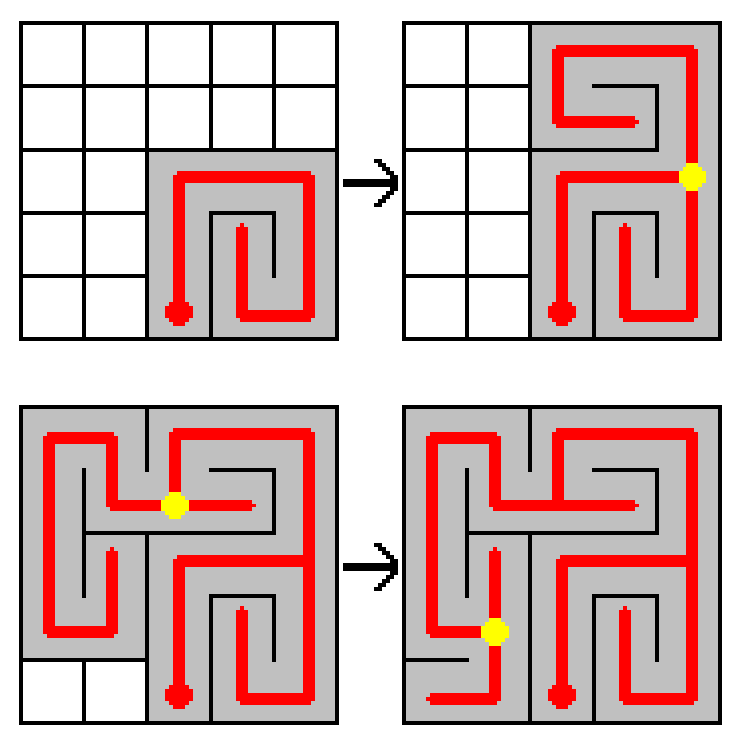
\includegraphics[scale=0.4]{fotos/back_tracker.png}
	\caption{Ejemplo de un algoritmo recursive backtracker \cite{back_tracker}}
	\label{back_tracker}
\end{figure}



\subsection{Programación del algoritmo}
\subsubsection{Recursivo}

Desde el punto de vista recursivo, esta forma de contruir un laberinto no presenta grandes problemas. El algoritmo crea una rama del laberinto hasta que le es imposible seguir porque, por ejemplo, el extremo ha quedado ``encerrado'' entre el muro exterior (el cual marca el límite y evita que el programa se salga de la memoria reservada para el laberinto evitando que el S.O. interrumpa la ejecución) y la propia rama. La naturaleza de la recursividad hace que, una vez llegado a ese punto, al no haber posibilidad de movimiento, resuelva por fin esa llamada a la función recursiva y devuelva el resultado a las casillas anteriores que aún estaban pendientes de resolución.  Esto continúa hasta que encuentra una casilla desde la que puede continuar camino, entonces abrirá desde ahí una nueva subrama del laberinto que continuará hasta que quede ``encerrada'' de nuevo y empiece a resolver hacia las casillas anteriores. Puede verse un ejemplo de dicha iteración en la figura \ref{back_tracker}. Finalmente, cuando ya no hay más casillas posibles por las que continuar, se volverá hacia atrás todas las casillas hasta llegar a la primera, en nuestro casi siempre la posición $(1,1)$. Este proceso asegura que el laberinto discurra por todas las casillas que sean posibles y que nunca quede encajonado" (como ya hemos dicho, la propia naturaleza de la recursividad lo garantiza).

\subsubsection{Iterativo}

El abordaje iterativo de este problema no es tan sencillo. Esto es debido, al hecho de que crear una rama principal de forma iterativa resulta más complejo que crearla recursivamente. Estableciendo unas condiciones lógicas de control para que la rama no se salga de los bordes y se evite a si misma para no romper el laberinto es suficiente. Pero tarde o temprano, la rama choca consigo misma y no tiene a donde ir. Solucionar este único punto es lo que más esfuerzo supone en la implementación del caso iterativo. La solución más inmedita resulta de crear un nuevo objeto o variable que almacene los lugares por los que la rama (o subrama) ya ha pasado. En esta memoria ha sido la última opción valorada, dado que su implementación significa alejarse del esquema marcado por el algoritmo recursivo. Para ello el equipo se dividió en dos: 
\begin{itemize}
	\item Una persona intentaría resolver el problema mediante la declaración de una variable dinámica local bidimensional. Es decir, una matriz con tantas filas como elementos tuviera la matriz sobre la que se hacía el laberinto y con tantas columnas como las dimensiones del laberinto (2 por ser bidimensional). 
	\item Otra persona intentaría la implementación de una pila dinámica tipo LIFO, que en un principio solo almacenaría los índices de las casillas por las que la rama o subrama había pasado en orden (más tarde se utilizó la pila también para almacenar más datos). 
	\item La tercera persona del equipo ejercería una labor de control y apoyo. Trabajando con las otras dos personas en limpieza del código e implementación de funciones auxiliares. Asimismo, controlaba el desarrollo de las dos vías con el fin de descartar la que menos conveniera para centrar todos los esfuerzos en la más prometedora.
\end{itemize}

Finalmente, la opción elegida fue la pila.  

En la primera versión solo almacenaba la situación de las casillas ya ocupadas por la rama. Posteriormente se incluyó una funcionalidad extra en el código: cuando el programa se viera obligado a retroceder por la rama que acababa de construir, comprobaría cada dirección de la casilla en la que estuviera para decidir si era posible continuar en alguna otra dirección, pero de forma que se incuría en algunas ineficiencias, pues se comprobaban direcciones que ya se habían comprobado antes, cuando la rama había pasado por allí por primera vez (o por segunda, o por tercera). Se almacenó entonces en la pila el vector de direcciones aleatorizado, así como por qué iteración iba la comprobación del vector. De esta forma es posible finalizar el laberinto asegurando que todas las direcciones han sido comprobadas y todas en un orden aleatorio.

\subsubsection{Comentarios al código}

Teniendo nuestros dos algoritmos finalizados, solo quedaba arreglar pequeños detalles como que el número de filas como de columnas debía ser impar. Ya que, por la manera de recorrer la malla de nuestros algoritmos, comprobando y avanzando de una en una sus casillas, si el número de estas fuese par, dejaría unos bordes izquierdo e inferior de dobles ‘\#’.  Este ‘arreglo’ se podía implementar de muchas maneras, una de ellas con una macro. Sin embargo, pensamos que era más sencillo incorporarla con dos líneas al final de nuestra función Pedir, que suman uno al número de filas o columnas en el caso de que sean pares. 

Por motivos estéticos, también decidimos buscar algún carácter en unicode para que las casillas no vaciadas de nuestros laberintos se asemejaran más a paredes y poder visualizar el dibujo más fácilmente. Encontramos el (insertar carácter) e implementando las siguientes líneas de código (que se encuentran comentadas en los ficheros correspondientes (nombreficheros/funciondonde estan) se puede apreciar que el laberinto queda mucho más intuitivo y agradable a la vista.  
\clearpage
\section{Experimentación}

\clearpage
\section{Análisis}

\clearpage
\section{Conclusiones}

\clearpage
\bibliographystyle{abbrv}
\bibliography{mybib}

\end{document}

